\documentclass[a4paper]{scrreprt}

% Uncomment to optimize for double-sided printing.
% \KOMAoptions{twoside}

% Set binding correction manually, if known.
% \KOMAoptions{BCOR=2cm}

% Localization options
\usepackage[english]{babel}
\usepackage[T1]{fontenc}
\usepackage[utf8]{inputenc}

% Quotations
\usepackage{dirtytalk}

% Floats
\usepackage{float}

% Enhanced verbatim sections. We're mainly interested in
% \verbatiminput though.
\usepackage{verbatim}

% Automatically remove leading whitespace in lstlisting
\usepackage{lstautogobble}

% PDF-compatible landscape mode.
% Makes PDF viewers show the page rotated by 90°.
\usepackage{pdflscape}

% Advanced tables
\usepackage{array}
\usepackage{tabularx}
\usepackage{longtable}

% Fancy tablerules
\usepackage{booktabs}

% Graphics
\usepackage{graphicx}

% Current time
\usepackage[useregional=numeric]{datetime2}

% Float barriers.
% Automatically add a FloatBarrier to each \section
\usepackage[section]{placeins}

% Custom header and footer
\usepackage{fancyhdr}

\usepackage{geometry}
\usepackage{layout}

% Math tools
\usepackage{mathtools}
% Math symbols
\usepackage{amsmath,amsfonts,amssymb}
\usepackage{amsthm}
% General symbols
\usepackage{stmaryrd}

\DeclarePairedDelimiter\abs{\lvert}{\rvert}

% Indistinguishable operator (three stacked tildes)
\newcommand*{\diffeo}{% 
  \mathrel{\vcenter{\offinterlineskip
  \hbox{$\sim$}\vskip-.35ex\hbox{$\sim$}\vskip-.35ex\hbox{$\sim$}}}}

% Bullet point
\newcommand{\tabitem}{~~\llap{\textbullet}~~}

\pagestyle{plain}
% \fancyhf{}
% \lhead{}
% \lfoot{}
% \rfoot{}
% 
% Source code & highlighting
\usepackage{listings}

% SI units
\usepackage[binary-units=true]{siunitx}
\DeclareSIUnit\cycles{cycles}

% Convenience commands
\newcommand{\mailsubject}{11043 - Internet of Things - Series 8}
\newcommand{\maillink}[1]{\href{mailto:#1?subject=\mailsubject}
                               {#1}}

% Should use this command wherever the print date is mentioned.
\newcommand{\printdate}{\today}

\subject{11043 - Internet of Things}
\title{Series 8}

\author{Michael Senn \maillink{michael.senn@students.unibe.ch} - 16-126-880}

\date{\printdate}

% Needs to be the last command in the preamble, for one reason or
% another. 
\usepackage{hyperref}

\begin{document}
\maketitle


\setcounter{chapter}{7}

\chapter{Series 8}

\section{Proactive vs reactive routing}

With proactive routing, routing tables are established ahead of time, before a
packet is meant to be transmitted. Routes are updated constantly. The advantage
is that, when a packet is to be sent, a route is immediately available. This
reduces latency, and improves throughput as a route can be reused for many
packets.

With reactive routing, a route is established on-demand when a packet is meant
to be transmitted. This increases latency and decreases throughput, as
transmission has to wait for the route to be established and a route cannot be
reused arbitrarily often. However it is more resistant to topology changes, as
the route is established right before the packet is sent, so is much more
likely to be available still.

As such, proactive routing is suitable in scenarios where the topology is
unlikely to change often, as might be the case in the backbone of a big
network. Reactive routing is more suited in a network where nodes may appear,
disappear and move at any time, such as a mesh network of many sensor nodes.

\section{Packet loss in WSN}

Assuming a packet loss rate in each direction of \SI{12}{\percent}, the
probability for a non-successful packet transmission follows as:
\[
		p = 1 - (1 - p_f) \cdot (1 - p_r) = 1 - (1 - 0.12)^2 = 0.2256 = \SI{22.56}{\percent}
\]

And the probability for a successful packet delivery on the fifth attempt as:
\[
		s(5) = 0.2256^4 \cdot (1 - 0.2256) \approx 0.002 = \SI{0.2}{\percent}
\]

\section{GPSR routing}

Given the provided network, GPSR routing from the source to the destination
will take place as follows. The text over each arrow indicates whether routing
happened \textbf{g}reedily (getting closer to the destination) or via
\textbf{p}ermieter routing (moving away from the destination node due to an
obstacle).

Assume that the distance JD is shorter than KD. In the exercise they are equal
to within a few pixels.

\[
		S \xrightarrow{g} B \xrightarrow{g} D \xrightarrow{g} F \xrightarrow{g}
		G \xrightarrow{p} E \xrightarrow{p} I \xrightarrow{p} K \xrightarrow{g}
		J \xrightarrow{p} K \xrightarrow{p} L \xrightarrow{p} M \xrightarrow{p}
		N \xrightarrow{g} D
\]

The path is also crudely visualized in figure \ref{fig:gpsr_routing}. Blue hops
are greedy, red are perimeter (with the counter-clockwise search direction
indicated).  The green line is the source-destination intersect which perimeter
hops may not cross.

\begin{figure}[h]
        \centering
        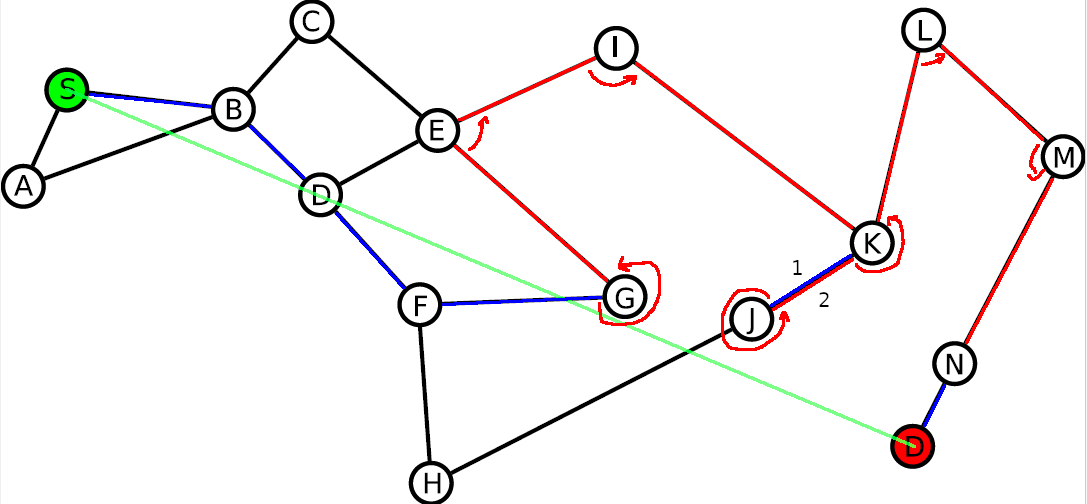
\includegraphics[width=\textwidth]{network}
        \caption{GPSR routing}
        \label{fig:gpsr_routing}
\end{figure}


\end{document}
